%------------------------------------------------------------------------------------
\clearpage
\begin{center}
  \textbf{\large 2. ПРАКТИЧЕСКАЯ ЧАСТЬ}
\end{center}
\refstepcounter{chapter}
\addcontentsline{toc}{chapter}{2. ПРАКТИЧЕСКАЯ ЧАСТЬ}
%------------------------------------------------------------------------------------

Для исследования влияния доплеровского масштабирования спектра на производительность системы,
использующей OFDM-модуляцию, было проведено численное моделирование. В ходе моделирования были
рассмотрены два случая: система, в которой не учитываются особенности стандарта 5G NR NTN по
выделению частотных ресурсов, и система, которая соответствует стандарту 5G NR NTN.

\section{Моделирование без учёта спецификации 5G NR NTN}

Рассмотрим несогласованный со спецификацией случай. На рис.~\ref{fig:ber_epsilon_scan_1024} 
показаны кривые зависимости вероятности битовой ошибки (BER)
от отношения сигнал/шум (SNR) для системы связи с модуляциями ФМ-4, КАМ-16, КАМ-64, КАМ-256
и количеством поднесущих $N = 1024$ для различных значений модуля относительной скорости приёмника и передатчика.

%------------------------------------------------------------------------------------
%Figure
%------------------------------------------------------------------------------------
\begin{figure}[h]
    \centering
    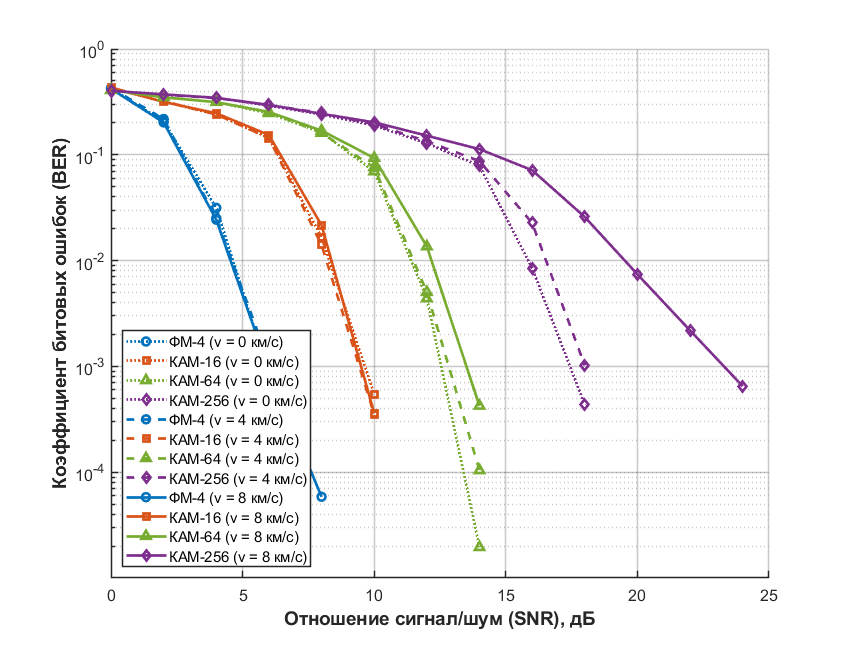
\includegraphics[width=1\textwidth]{images/res/ber_epsilon_scan_1024.png}
    \caption{Зависимость вероятности битовой ошибки (BER) от отношения сигнал/шум (SNR)
             для различных значений модуля относительной скорости при $N = 1024$}
    \label{fig:ber_epsilon_scan_1024}
\end{figure}
\FloatBarrier
%------------------------------------------------------------------------------------

Из графика видно, что влияние эффекта масштабирования спектра для $N = 1024$ начинает проявляться
для типов модуляции КАМ-64 и КАМ-256. Для КАМ-64 наблюдается отклонение порядка $\sim 1$ дБ при $V = 8$ км/с.
Для КАМ-256 отклонения при $V = 4$ км/с составляют порядка $\sim 1$ дБ, а для $V = 8$ км/с кривые различаются 
на $2.5$ дБ при $\text{BER} \sim 10^{-3}$.

На рис.~\ref{fig:ber_epsilon_scan_2048} 
показаны кривые зависимости вероятности битовой ошибки (BER)
от отношения сигнал/шум (SNR) для системы связи с количеством поднесущих $N = 2048$
для различных значений модуля относительной скорости приёмника/передатчика.

%------------------------------------------------------------------------------------
%Figure
%------------------------------------------------------------------------------------
\begin{figure}[h]
    \centering
    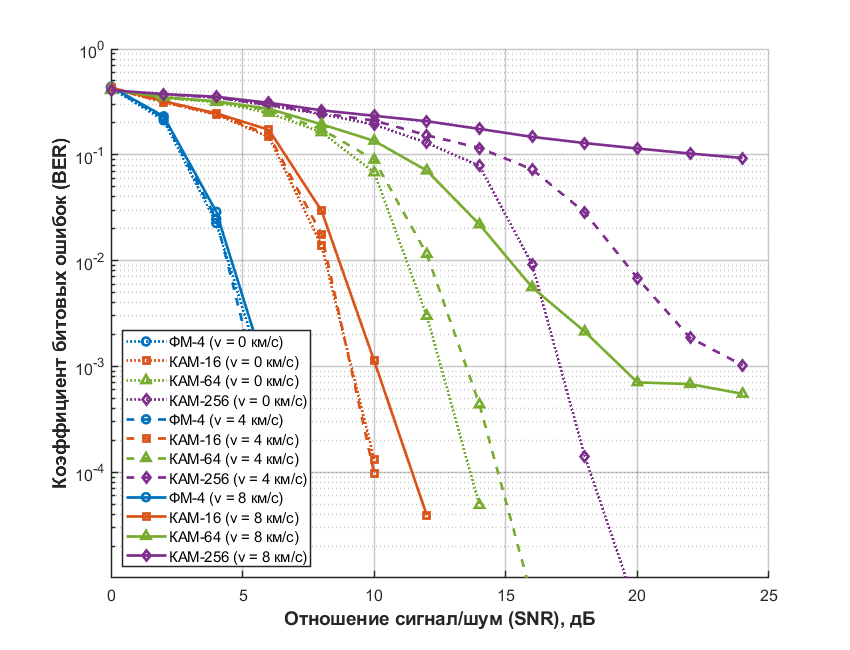
\includegraphics[width=1\textwidth]{images/res/ber_epsilon_scan_2048.png}
    \caption{Зависимость вероятности битовой ошибки (BER) от отношения сигнал/шум (SNR)
             для различных значений модуля относительной скорости при $N = 2048$}
    \label{fig:ber_epsilon_scan_2048}
\end{figure}
\FloatBarrier
%------------------------------------------------------------------------------------

В данном случае с увеличением количества поднесущих существенно возрастает уровень интерференции между поднесущими (ICI), что 
приводит к ухудшению характеристик системы. Для модуляции КАМ-16 наблюдается различие в $\sim 1$ дБ при уровне
$\text{BER} = 10^{-3}$. Для КАМ-64 при $V = 8$ км/с и КАМ-256 при $V = 4$ км/с уровень расхождения достигает $7$ дБ.

\newpage
На рис.~\ref{fig:ber_fft_scan_raw} показаны кривые зависимости вероятности битовой ошибки (BER)
от отношения сигнал/шум (SNR) для OFDM-сигнала с различными видами модуляции и модулем относительной скорости 
$V = 8$ км/с для различных значений количества поднесущих.

%------------------------------------------------------------------------------------
% Figure
%------------------------------------------------------------------------------------
\begin{figure}[h]
    \centering
    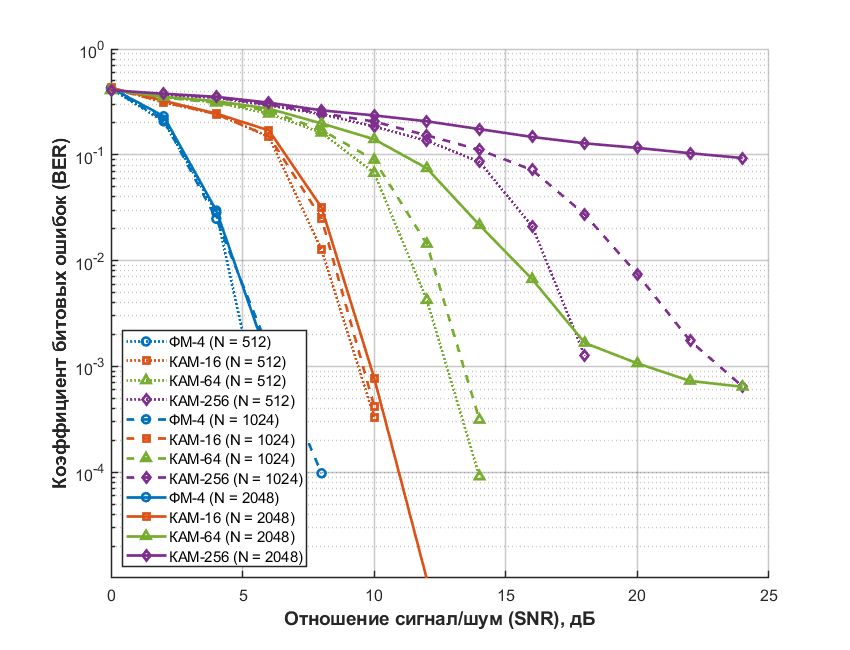
\includegraphics[width=1\textwidth]{images/res/ber_fft_scan_raw.png}
    \caption{Зависимость вероятности битовой ошибки (BER) от отношения сигнал/шум (SNR)
             для различных значений количества поднесущих при $V = 8$ км/с}
    \label{fig:ber_fft_scan_raw}
\end{figure}
\FloatBarrier
%------------------------------------------------------------------------------------

Из представленных данных следует, что при параметрах $N = 2048$ и $V = 8$ км/с модуляция КАМ-256
демонстрирует полную неработоспособность, а для КАМ-64 фиксируется падение помехозащищен\-ности на $7$
 дБ. При $N = 1024$, $V = 4$ км/с КАМ-256 расходится относительно 
кривой с $N = 512$ на $7$ дБ, КАМ-64 и КАМ-16 расходятся на величину $\sim 1$ дБ.

\section{Моделирование с учётом спецификации 5G NR NTN}

Рассмотрим случай, когда в системе используется способ частотного выделения, указанный в спецификации.
На рис.~\ref{fig:ber_epsilon_scan_5g} 
показаны кривые зависимости вероятности битовой ошибки (BER)
от отношения сигнал/шум (SNR) для системы связи с различными видами модуляции
и количеством поднесущих $N = 2048$ (для определённого количества ресурсных блоков) для различных значений модуля относительной 
скорости приёмника/передатчика.

%------------------------------------------------------------------------------------
% Figure
%------------------------------------------------------------------------------------
\begin{figure}[h]
    \centering
    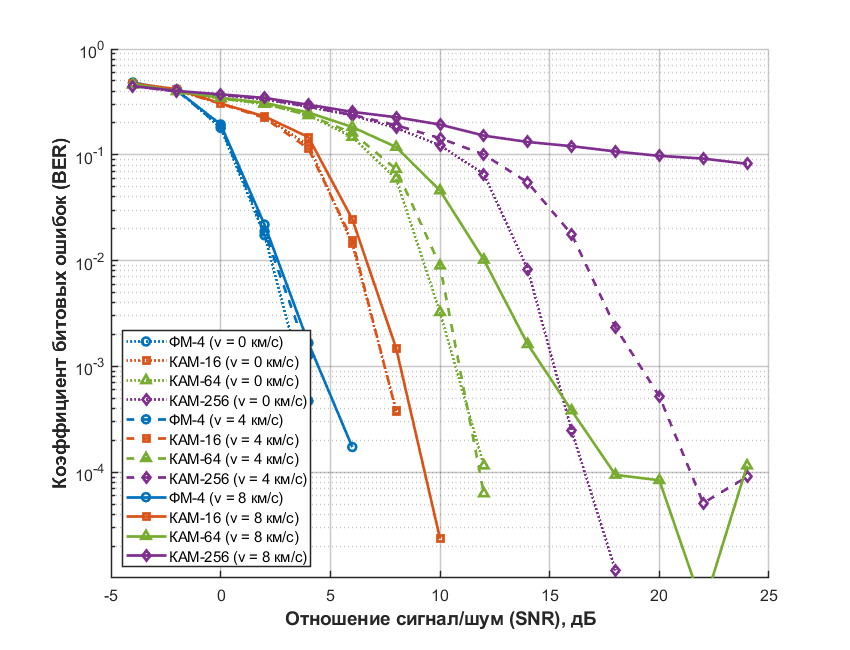
\includegraphics[width=1\textwidth]{images/res/ber_epsilon_scan_5g.png}
    \caption{Зависимость вероятности битовой ошибки (BER) от отношения сигнал/шум (SNR)
             для различных значений модуля относительной скорости при $N = 2048$ и соответствующем количестве ресурсных блоков}
    \label{fig:ber_epsilon_scan_5g}
\end{figure}
\FloatBarrier
%------------------------------------------------------------------------------------

По сравнению с рис.~\ref{fig:ber_epsilon_scan_2048} данная система испытывает 
меньшее ухудшение производительности. В данном случае влияние масштабирования на ФМ-4 и КАМ-16 
является незначительным. Для остальных случаев наблюдаются расхождения: КАМ-64 при $V = 4$ км/с
смещена на $1$ дБ, при $V = 8$ км/с - на $4$ дБ; КАМ-256 при $V = 4$ км/с смещена на $3$ дБ, при
$V = 8$ км/с выходит на плато (ошибки перестают уменьшаться с ростом SNR) и не может успешно демодулировать пакеты.

\newpage
На рис.~\ref{fig:ber_fft_scan_5g} показаны кривые зависимости вероятности битовой ошибки (BER)
от отношения сигнал/шум (SNR) для OFDM-сигнала с различными видами модуляции и модулями относительной скорости 
$V = 0$ и $8$ км/с для различных значений количества ресурсных блоков.

%------------------------------------------------------------------------------------
% Figure
%------------------------------------------------------------------------------------
\begin{figure}[h]
    \centering
    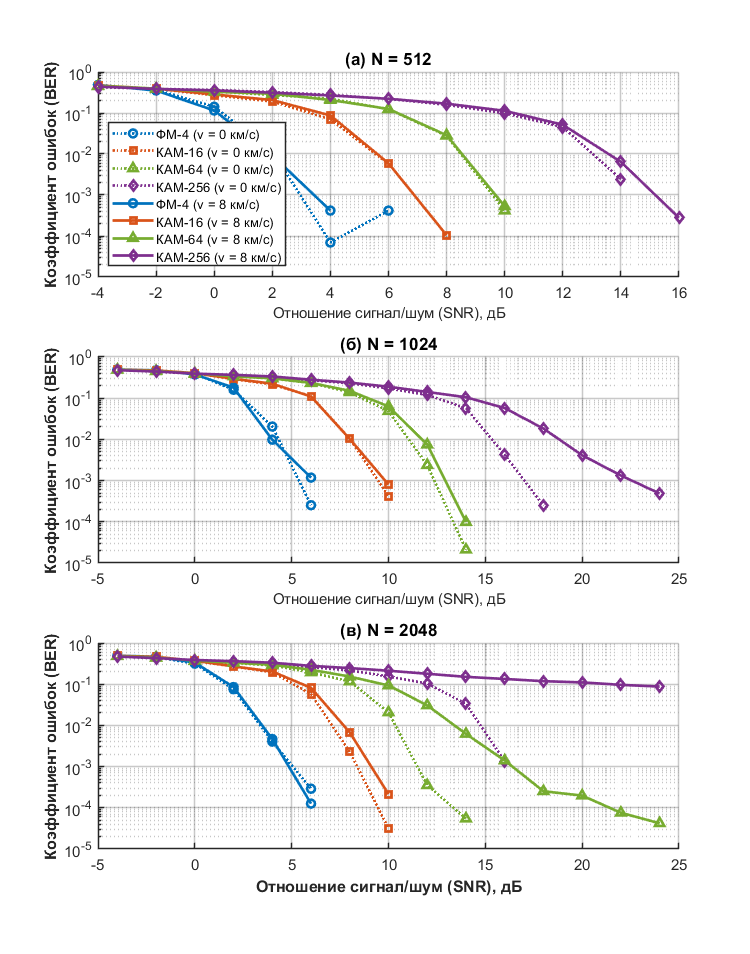
\includegraphics[width=1.1\textwidth]{images/res/ber_fft_scan_5g.png}
    \caption{Зависимость вероятности битовой ошибки (BER) от отношения сигнал/шум (SNR)
             для различных значений количества ресурсных блоков. 
             Система соответствует частотному выделению спецификации 5G NR}
    \label{fig:ber_fft_scan_5g}
\end{figure}
\FloatBarrier
%------------------------------------------------------------------------------------

Из графика (рис.~\ref{fig:ber_fft_scan_5g}а) видно, что масштабирование спектра при $N = 512$ на данную систему не вносит существенного влияния.
На графике (рис.~\ref{fig:ber_fft_scan_5g}б) можно заметить влияние ICI только для КАМ-256 (смещение на $\sim 5$ дБ). 
На графике (рис.~\ref{fig:ber_fft_scan_5g}в) влияние ICI сказывается на КАМ-64 и КАМ-256: в первом случае наблюдается смещение порядка $5$ дБ, а
во втором случае система не может корректно принимать пакеты.

Проведённое численное моделирование позволяет сделать следующие выводы о влиянии доплеровского 
масштабирования спектра на помехо\-устойчивость OFDM-систем в контексте стандарта 5G NR NTN.

\begin{enumerate}
    \item \textbf{Существенность эффекта для высокоскоростных сценариев.} 
    Доплеровское масштабирование спектра приводит к заметному ухудшению помехоустойчивости при 
    скоростях относительного движения от $4$ км/с и выше. Наиболее сильно эффект проявляется для 
    высокоуровневых модуляций (КАМ-64, КАМ-256) и при большом количестве поднесущих ($N=2048$), 
    где интерференция между поднесущими (ICI) становится доминирующим фактором.

    \item \textbf{Влияние количества поднесущих.} 
    Увеличение числа поднесущих при фиксированной относительной скорости приводит к усилению ICI.
    Для $N=2048$ и $V=8$ км/с модуляция КАМ-256 оказывается полностью неработоспособной,
    а для КАМ-64 потери в SNR достигают $7$ дБ по сравнению с идеальным каналом.
    Для $N=512$ влияние масштабирования существенно меньше.

    \item \textbf{Ограничения для высоких модуляций.} 
    Даже при использовании спецификационных подходов частотного выделения модуляции выше КАМ-64 оказываются крайне 
    чувствительными к доплеровскому масштабированию. Для КАМ-256 при $V = 8$ км/с наблюдается выход BER на плато,
     что делает такие модуляции непригодными для спутниковых каналов 
    LEO без дополнительной компенсации.

\end{enumerate}